\section{Backend}

\subsection{Tecnologies and libraries}

\subsubsection{NodeJs}
Node.js is an open-source, cross-platform, back-end JavaScript runtime environment that runs on the V8 engine and executes JavaScript code outside a web browser. Node.js lets developers use JavaScript to write command line tools and for server-side scripting—running scripts server-side to produce dynamic web page content before the page is sent to the user's web browser. Consequently, Node.js represents a "JavaScript everywhere" paradigm, unifying web-application development around a single programming language, rather than different languages for server-side and client-side scripts.

\begin{itemize}
    \item \textbf{Used Version:} 4.2.2 
\end{itemize}

\subsubsection{Typescript}
TypeScript is a programming language developed and maintained by Microsoft. It is a strict syntactical superset of JavaScript and adds optional static typing to the language. TypeScript is designed for the development of large applications and transcompiles to JavaScript. 
   
    \begin{itemize}
        \item \textbf{Used Version:} 4.2.2 
    \end{itemize}

\subsubsection{JSON}
JSON (JavaScript Object Notation) is an open standard file format, and data interchange format, that uses human-readable text to store and transmit data objects consisting of attribute–value pairs and array data types (or any other serializable value). It is a very common data format, with a diverse range of applications, such as serving as a replacement for XML in AJAX systems.


\subsubsection{DynamoDB}
Amazon DynamoDB is a fully managed proprietary NoSQL database service that supports key-value and document data structures and is offered by Amazon.com as part of the Amazon Web Services portfolio
\subsubsection{Npm}
npm is the package manager for the Node JavaScript platform. It puts modules in place so that node can find them, and manages dependency conflicts intelligently.
It is extremely configurable to support a wide variety of use cases. Most commonly, it is used to publish, discover, install, and develop node programs.
\subsubsection{Swagger}
Swagger is an Interface Description Language for describing RESTful APIs expressed using JSON. Swagger is used together with a set of open-source software tools to design, build, document, and use RESTful web services. Swagger includes automated documentation, code generation (into many programming languages), and test-case generation.


\subsection{Sequence diagrams}
In this section we'll provide sequence diagrams for explaining how microservices communicates between each others
when certains API's are called from the fronend service.

\subsubsection{Checkout}
\begin{figure}[H]
    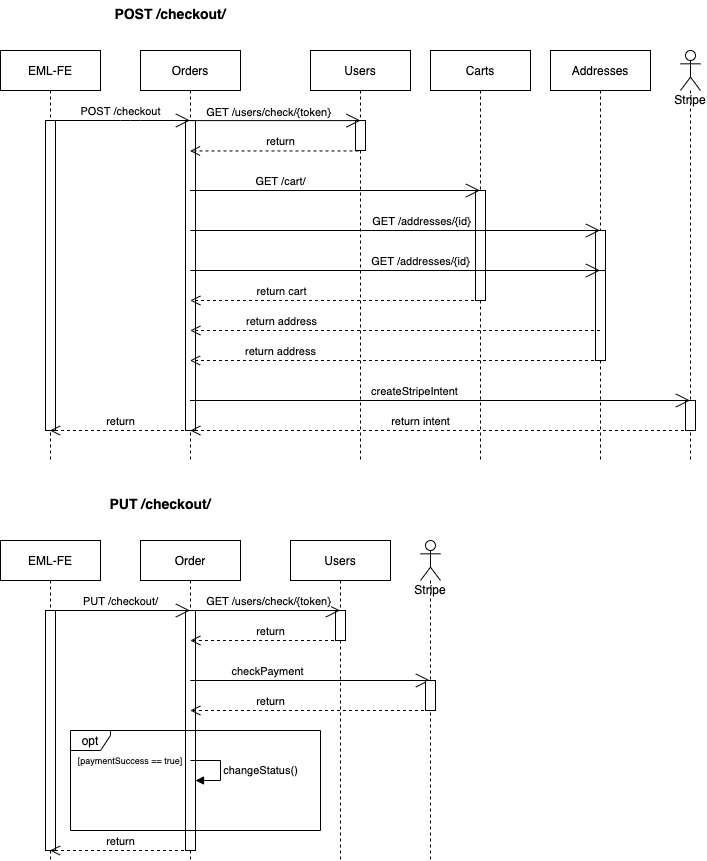
\includegraphics[width=0.9\textwidth]{res/images/sequence-diagrams/checkout.jpg}
\end{figure}

\subsubsection{Carts}
\begin{figure}[H]
    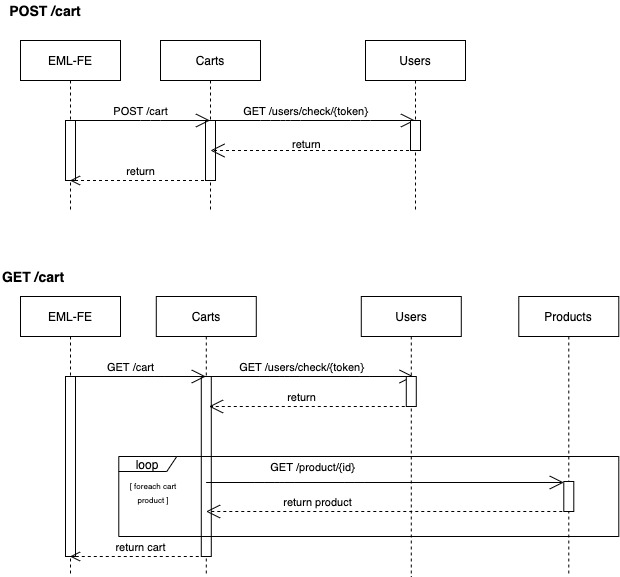
\includegraphics[width=0.9\textwidth]{res/images/sequence-diagrams/carts.jpg}
\end{figure}

\subsubsection{Products}
\begin{figure}[H]
    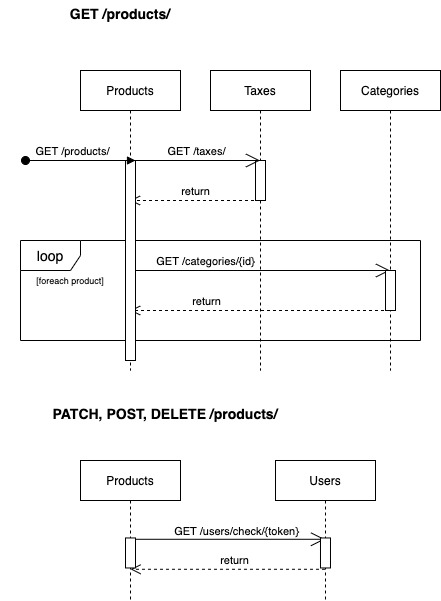
\includegraphics[width=0.7\textwidth]{res/images/sequence-diagrams/products.jpg}
\end{figure}